\section{Results in the finite mazes}\label{sec:results-finite}

This section answers the performance and stability parts of Q4; the sample and compute requirements are in \cref{sec:costs}.
All quantities are exact oracle values for the policy at the last checkpoint, i.e.\ after the full budget, reported as mean and sample standard deviation over the seeds $0$, $1$, $2$; every seed is listed in \cref{app:results}.
The Monte Carlo cross-checks agree with the exact values and are not repeated.

\subsection{Experts and the demonstration target}

The six experts are optimal for their evaluation rewards: their gap to $V^\star_H$ is $\vn{s11.expert_gap}{0}$, and $V^\star_H$ at the start is $\vn{s11.V.open.side}{15.51}$ (open) or $\vn{s11.V.4r.side}{15.53}$ (four rooms) for the goals $(5,1)$ and $(1,5)$, and $\vn{s11.V.open55}{12.43}$ (open) or $\vn{s11.V.4r55}{12.36}$ (four rooms) for $(5,5)$.
An expert reaches its goal in every episode and then stays there: its next-state occupancy $q_E$ puts $\vn{s11.goalmass.lo}{0.61}$--$\vn{s11.goalmass.hi}{0.77}$ of its mass on the goal cell, and the probability that $s_H$ lies in the goal is $\vn{s11.expert_fig}{0.916}$.
To imitate it, a policy must therefore reach the goal quickly \emph{and stay}; reaching it is what the success rate measures, staying is what the return and the divergence measure.

The learners never see $q_E$. $f$-PG matches the smoothed empirical occupancy $\hat q_E$ of the four demonstrations, \ERFB{} and \DMFB{} use the same demonstration states. That target is itself at a held-out divergence $\JS(\hat q_E,q_E)$ of $\vn{s11.demo_target.lo}{0.007}$ to $\vn{s11.demo_target.hi}{0.022}$ nats from the expert. All held-out divergences below are computed against the exact $q_E$.

\subsection{Final performance}

\begin{table}[ht]
\centering\small
\caption{Finite mazes, core suite, last checkpoint (mean $\pm$ sample SD over 3 seeds). JS is the held-out next-state occupancy divergence $\JS(d^+_{\pi,H},q_E)$, success the exact probability of reaching the goal within $H$ steps, the gap is $V^\star_H-J_H(\pi)$ for the evaluation reward, and $\JS^{\SA}$ the state--action diagnostic. Generated from the run files by \texttt{report/verify/make\_tables.py}.}\label{tab:finite}
\resizebox{\textwidth}{!}{% GENERATED by report/verify/make_tables.py from the saved run files (runs/jobs/*).
% Finite mazes, core suite: final held-out metrics, mean +/- sample SD over seeds 0, 1, 2.
% Do not edit by hand: rerun  python3 report/verify/verify_results.py

\begin{tabular}{@{}llrcccc@{}}
\toprule
layout, goal & method & $V^\star_H$ & JS (nats) & success & gap to $V^\star_H$ & $\JS^{\SA}$ (nats)\\
\midrule
open (5,1) & \fPG{} (JS) & 15.51 & $0.010\pm0.014$ & $1.000\pm0.000$ & $0.63\pm0.50$ & $0.026\pm0.020$\\
 & \DMFB &  & $0.535\pm0.082$ & $0.218\pm0.221$ & $14.35\pm0.89$ & $0.572\pm0.086$\\
 & \ERFB &  & $0.437\pm0.013$ & $0.868\pm0.128$ & $13.49\pm0.51$ & $0.532\pm0.003$\\
\addlinespace
open (5,5) & \fPG{} (JS) & 12.43 & $0.019\pm0.014$ & $1.000\pm0.000$ & $1.36\pm1.15$ & $0.065\pm0.045$\\
 & \DMFB &  & $0.457\pm0.051$ & $0.450\pm0.081$ & $11.00\pm0.31$ & $0.507\pm0.055$\\
 & \ERFB &  & $0.292\pm0.074$ & $0.992\pm0.012$ & $8.65\pm2.24$ & $0.418\pm0.067$\\
\addlinespace
open (1,5) & \fPG{} (JS) & 15.51 & $0.002\pm0.001$ & $1.000\pm0.000$ & $0.35\pm0.18$ & $0.012\pm0.004$\\
 & \DMFB &  & $0.397\pm0.252$ & $0.441\pm0.477$ & $11.68\pm4.39$ & $0.441\pm0.228$\\
 & \ERFB &  & $0.339\pm0.213$ & $0.808\pm0.293$ & $11.03\pm4.09$ & $0.433\pm0.220$\\
\addlinespace
four rooms (5,1) & \fPG{} (JS) & 15.53 & $0.002\pm0.000$ & $1.000\pm0.000$ & $0.39\pm0.21$ & $0.009\pm0.003$\\
 & \DMFB &  & $0.589\pm0.049$ & $0.087\pm0.042$ & $15.09\pm0.33$ & $0.620\pm0.047$\\
 & \ERFB &  & $0.436\pm0.011$ & $0.944\pm0.027$ & $13.87\pm0.21$ & $0.530\pm0.017$\\
\addlinespace
four rooms (5,5) & \fPG{} (JS) & 12.36 & $0.015\pm0.005$ & $1.000\pm0.000$ & $1.44\pm0.34$ & $0.048\pm0.019$\\
 & \DMFB &  & $0.476\pm0.204$ & $0.327\pm0.540$ & $11.38\pm1.64$ & $0.550\pm0.183$\\
 & \ERFB &  & $0.348\pm0.109$ & $0.772\pm0.196$ & $10.25\pm1.78$ & $0.425\pm0.085$\\
\addlinespace
four rooms (1,5) & \fPG{} (JS) & 15.53 & $0.006\pm0.006$ & $0.999\pm0.001$ & $0.68\pm0.34$ & $0.016\pm0.008$\\
 & \DMFB &  & $0.365\pm0.226$ & $0.628\pm0.505$ & $11.50\pm3.71$ & $0.421\pm0.219$\\
 & \ERFB &  & $0.278\pm0.181$ & $0.936\pm0.094$ & $9.95\pm4.99$ & $0.364\pm0.223$\\
\bottomrule
\end{tabular}
}
\end{table}

\Cref{tab:finite} and \cref{fig:final-core} summarize the final policies.

\paragraph{$f$-PG} ends close to the expert in every run: the held-out divergence is $\vn{s11.fpg.js.lo}{0.0011}$ to $\vn{s11.fpg.js.hi}{0.032}$ nats, the success probability at least $\vn{s11.fpg.succ_min}{0.998}$, the gap to $V^\star_H$ between $\vn{s11.fpg.gap.lo}{0.15}$ and $\vn{s11.fpg.gap.hi}{2.68}$, and the probability of ending in the goal $\vn{s11.fpg.fig.lo}{0.853}$ to $\vn{s11.fpg.fig.hi}{0.912}$ against the expert's $\vn{s11.expert_fig}{0.916}$.
The final policies are nearly deterministic on the states they visit (mean policy entropy $\vn{s11.fpg.ent.lo}{0.03}$ to $\vn{s11.fpg.ent.hi}{0.17}$ nats, against $\log5\approx\vn{const.log5}{1.61}$ for a uniform policy).

\paragraph{\ERFB} reaches the goal in most runs but rarely stays: success is $\vn{s11.er.succ.lo}{0.47}$ to $\vn{s11.er.succ.hi}{1.00}$, and at least $0.80$ in \vn{s11.er.n08}{14} of the \vn{n.runs.finite}{18} runs, but the probability of ending in the goal is $\vn{s11.er.fig.lo}{0.001}$ to $\vn{s11.er.fig.hi}{0.51}$ (at least $0.5$ in \vn{s11.er.fig05}{a single} run), the gap is $\vn{s11.er.gap.lo}{4.3}$ to $\vn{s11.er.gap.hi}{14.1}$, and the held-out divergence is $\vn{s11.er.js.lo}{0.079}$ to $\vn{s11.er.js.hi}{0.497}$ nats.
Under exactness \ERFB{} would maximize the reward $\dd\rho_e/\dd\nu$ (\cref{prop:m-er}), which is largest at the goal where the expert spends most of its time; the trained model does not deliver this.

\paragraph{\DMFB} is worse than \ERFB{} in almost every run: its divergence is $\vn{s11.dm.js.lo}{0.122}$ to $\vn{s11.dm.js.hi}{0.645}$ nats, its success $\vn{s11.dm.succ.lo}{0.0005}$ to $\vn{s11.dm.succ.hi}{0.975}$ (at least $0.80$ in \vn{s11.dm.n08}{4} runs), its gap $\vn{s11.dm.gap.lo}{6.7}$ to $\vn{s11.dm.gap.hi}{15.4}$.
Paired by layout, goal and seed, \DMFB{} has a larger divergence than \ERFB{} in \vn{s11.pair.js}{16} of the \vn{s11.pair.n}{18} runs and a lower success in \vn{s11.pair.succ}{17}. Since \DMFB{} starts from the \ERFB{} latent, this is a statement about what the 300 latent steps did; \cref{sec:m-dm-path} examines it.

\paragraph{State--action diagnostic.}
For every policy $\JS^{\SA}\ge\JS$, as it must be: $d^+_{\pi,H}$ is the image of $d^{\SA}_{\pi,H}$ under the kernel $P$, and an $f$-divergence cannot increase under a Markov kernel \citep{csiszar1967information}.
For $f$-PG the state--action divergence is $\vn{s11.fpg.jssa.lo}{0.006}$ to $\vn{s11.fpg.jssa.hi}{0.111}$ nats. State matching does not determine the expert's actions (\cref{ex:occ-blocked}), and we do not claim that $f$-PG recovers them.

\begin{figure}[t]
\centering
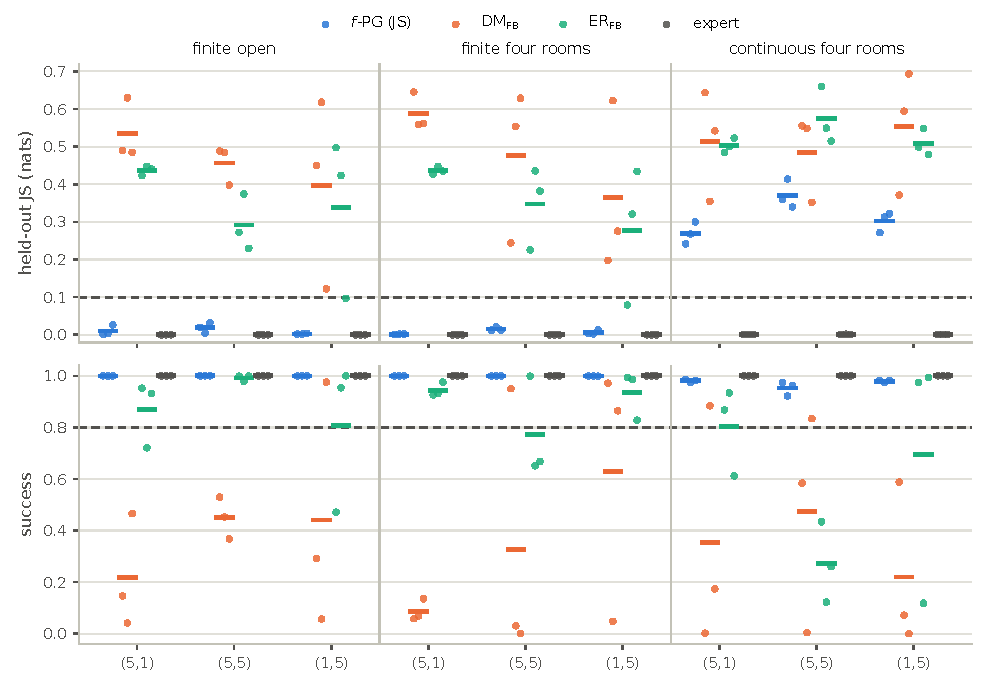
\includegraphics[width=\textwidth]{figures/fig_final_seeds.pdf}
\caption{Every core run at the last checkpoint, finite and continuous: held-out divergence (top) and success (bottom), with the operational thresholds (dashed). Dots are seeds, bars the means over the three seeds; the expert is the reference.}\label{fig:final-core}
\end{figure}

\subsection{Learning curves and the operational thresholds}

\begin{table}[ht]
\centering\small
\caption{Operational thresholds ($\JS\le0.10$ nats and success $\ge0.80$), declared before the runs: number of seeds that meet them at the last checkpoint, and the first assessed checkpoint at which each seed met them (``--'': at no assessed checkpoint within the budget; \DMFB{} is assessed after its completed latent steps). $f$-PG is counted in learner transitions, \ERFB{} and \DMFB{} in FB pretraining updates (the latent adaptation itself uses no transition).}\label{tab:convergence}
% GENERATED by report/verify/make_tables.py from the saved run files (runs/jobs/*).
% Operational thresholds JS <= 0.10 nats and success >= 0.80: seeds meeting them at the last checkpoint, and the first checkpoint at which each seed met them (seed order 0, 1, 2).
% Do not edit by hand: rerun  python3 report/verify/verify_results.py

\begin{tabular}{@{}lllcl@{}}
\toprule
maze & goal & method & met at last & first reached (seeds 0, 1, 2)\\
\midrule
finite open & (5,1) & \fPG{} (JS) & 3/3 & 20k, 20k, 20k (transitions)\\
 &  & \DMFB & 0/3 & --, --, 2.5k (FB updates)\\
 &  & \ERFB & 0/3 & 2.5k, --, -- (FB updates)\\
\addlinespace
 & (5,5) & \fPG{} (JS) & 3/3 & 20k, 20k, 20k (transitions)\\
 &  & \DMFB & 0/3 & --, --, -- (FB updates)\\
 &  & \ERFB & 0/3 & --, --, -- (FB updates)\\
\addlinespace
 & (1,5) & \fPG{} (JS) & 3/3 & 20k, 20k, 20k (transitions)\\
 &  & \DMFB & 0/3 & 2.5k, --, -- (FB updates)\\
 &  & \ERFB & 1/3 & --, --, 10k (FB updates)\\
\midrule
finite four rooms & (5,1) & \fPG{} (JS) & 3/3 & 20k, 20k, 20k (transitions)\\
 &  & \DMFB & 0/3 & --, --, -- (FB updates)\\
 &  & \ERFB & 0/3 & --, --, -- (FB updates)\\
\addlinespace
 & (5,5) & \fPG{} (JS) & 3/3 & 30k, 20k, 20k (transitions)\\
 &  & \DMFB & 0/3 & --, 5k, -- (FB updates)\\
 &  & \ERFB & 0/3 & --, --, -- (FB updates)\\
\addlinespace
 & (1,5) & \fPG{} (JS) & 3/3 & 20k, 20k, 20k (transitions)\\
 &  & \DMFB & 0/3 & 7.5k, 5k, -- (FB updates)\\
 &  & \ERFB & 1/3 & 10k, --, -- (FB updates)\\
\midrule
continuous & (5,1) & \fPG{} (JS) & 0/3 & --, --, -- (transitions)\\
 &  & \DMFB & 0/3 & --, --, -- (FB updates)\\
 &  & \ERFB & 0/3 & --, --, -- (FB updates)\\
\addlinespace
 & (5,5) & \fPG{} (JS) & 0/3 & --, --, -- (transitions)\\
 &  & \DMFB & 0/3 & --, --, -- (FB updates)\\
 &  & \ERFB & 0/3 & --, --, -- (FB updates)\\
\addlinespace
 & (1,5) & \fPG{} (JS) & 0/3 & --, --, -- (transitions)\\
 &  & \DMFB & 0/3 & --, --, -- (FB updates)\\
 &  & \ERFB & 0/3 & --, --, -- (FB updates)\\
\bottomrule
\end{tabular}

\end{table}

\begin{figure}[t]
\centering
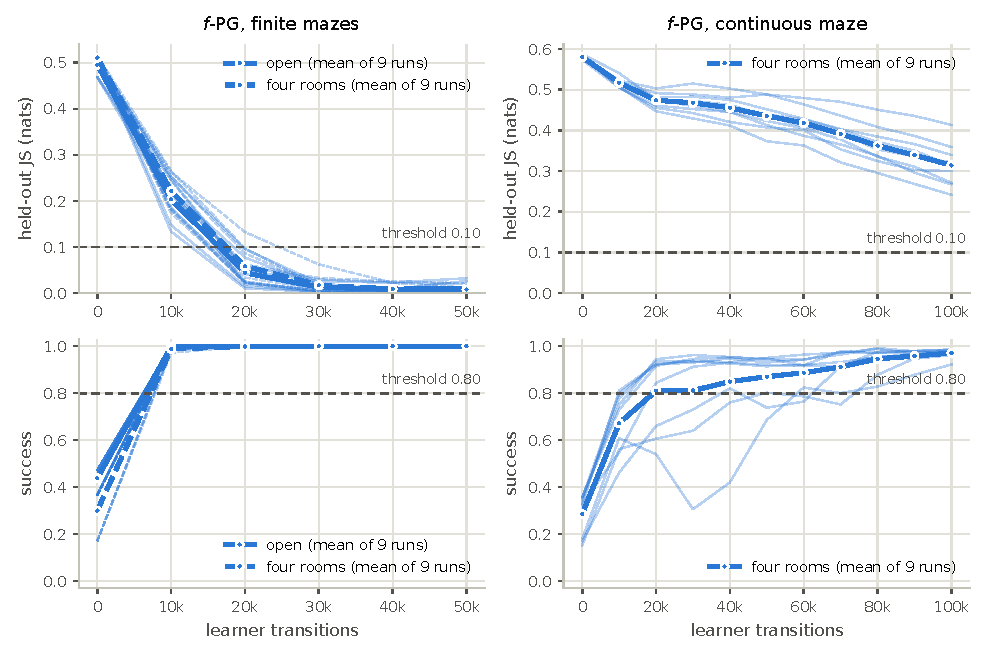
\includegraphics[width=\textwidth]{figures/fig_fpg_curves.pdf}
\caption{$f$-PG learning curves (core suite): held-out divergence and success against learner transitions. Thin lines are the individual runs, thick lines the mean over the \vn{n.fpg.per_maze}{9} runs of a maze (finite: open solid, four rooms dashed). The dashed horizontal lines are the operational thresholds.}\label{fig:fpg-curves}
\end{figure}

\begin{figure}[t]
\centering
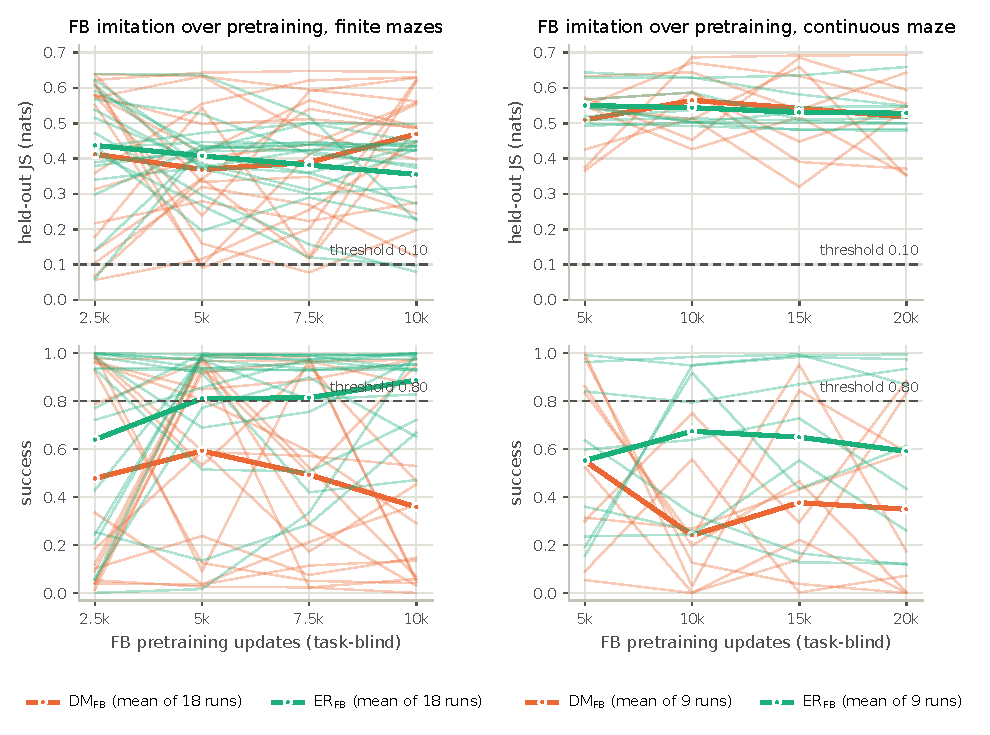
\includegraphics[width=\textwidth]{figures/fig_fbil_snapshots.pdf}
\caption{\ERFB{} and \DMFB{} (after its 300 latent steps) evaluated at every FB pretraining snapshot, against the number of task-blind pretraining updates. Thin lines are the runs, thick lines the means (finite: \vn{n.runs.finite}{18} runs per method; continuous: \vn{n.runs.cont}{9}).}\label{fig:fbil-snapshots}
\end{figure}

\paragraph{$f$-PG} (\cref{fig:fpg-curves}, left) starts from the uniform policy at a divergence of $\vn{s11.fpg.js0.lo}{0.47}$ to $\vn{s11.fpg.js0.hi}{0.52}$ nats and meets the thresholds in all \vn{abs.fpg.n}{18} runs, first at the $\vn{abs.fpg.first.lo}{20{,}000}$-transition checkpoint (\vn{s11.fpg.updates_at_20k}{10} policy updates) in \vn{s11.fpg.n20k}{17} runs and at the $\vn{abs.fpg.first.hi}{30{,}000}$-transition checkpoint in the remaining \vn{s11.fpg.n30k}{one} (four rooms, goal $(5,5)$, seed 0); all \vn{s11.fpg.last}{18} still meet them at the end of the budget (\cref{tab:convergence}).
With checkpoints every $\vn{fpg.interval.f}{10{,}000}$ transitions, these first hits are observed bounds at that resolution: the thresholds were first met somewhere between the previous checkpoint and this one.
The curves are smooth and every seed follows the mean closely.

\paragraph{\ERFB{} and \DMFB} (\cref{fig:fbil-snapshots}, left) behave differently. Their quality does not improve steadily with pretraining: between consecutive snapshots the held-out divergence of a run changes by up to $\vn{s11.swing}{0.53}$ nats, and \vn{s11.lost}{12} of the \vn{s11.curves}{36} finite curves reach a success of $0.80$ at an earlier snapshot but not at the last one.
\ERFB{} meets the thresholds at the last snapshot in \vn{abs.er.last}{2} runs (open, goal $(1,5)$, seed 2, and four rooms, goal $(1,5)$, seed 0), and in \vn{s11.er.early_n}{one} more run only at the first snapshot (open, goal $(5,1)$, seed 0, after $\vn{s11.er.early_first}{2{,}500}$ updates).
\DMFB{} meets them at some snapshot in \vn{s11.dm.ever}{5} runs, after $\vn{s11.dm.first0}{2{,}500}$, $\vn{s11.dm.first1}{2{,}500}$, $\vn{s11.dm.first2}{5{,}000}$, $\vn{s11.dm.first3}{5{,}000}$ and $\vn{s11.dm.first4}{7{,}500}$ updates, and at the last snapshot in \vn{abs.dm.last}{none}.
So \vn{s11.notlast}{34} of the \vn{s11.curves}{36} finite FB-imitation runs do not meet the thresholds at the end of the budget: \vn{s11.earlyonly}{6} of them met them at an earlier snapshot only, and \vn{s11.never}{28} did not meet the thresholds at any assessed FB snapshot after completed adaptation (\emph{not reached} in \cref{tab:convergence}).
Of these \vn{s11.never}{28} runs, \vn{s11.dm.mid_cross}{three} are \DMFB{} runs (open maze, goal $(1,5)$, seeds 1 and 2; open maze, goal $(5,1)$, seed 0) whose latent path at the final snapshot crossed both thresholds at an intermediate latent step and left the threshold region before the final step; counting every evaluated checkpoint, including these intermediate iterates, \vn{s11.never_any}{25} of the \vn{s11.curves}{36} runs, rather than \vn{s11.never}{28}, never met the thresholds. The convergence rule, which assesses \DMFB{} after its completed adaptation, is unchanged. Their full curves are in \cref{app:results}.

\subsection{Why \texorpdfstring{\DMFB}{DM-FB} moves away from the expert}\label{sec:m-dm-path}

\begin{figure}[t]
\centering
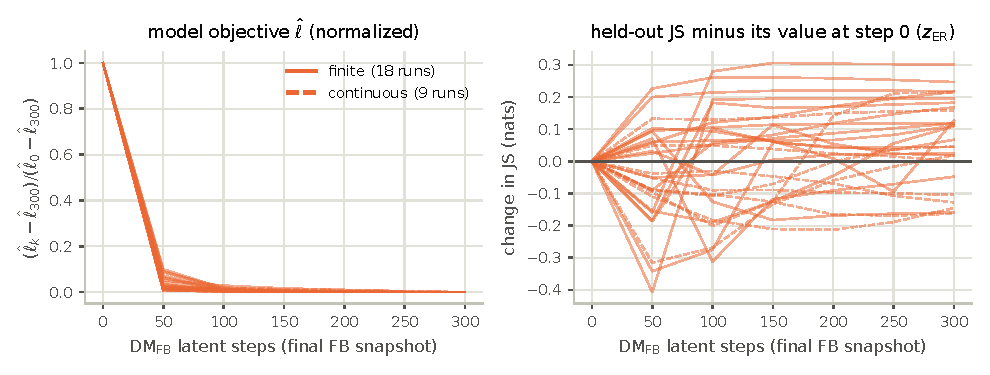
\includegraphics[width=\textwidth]{figures/fig_dm_path.pdf}
\caption{The 300 \DMFB{} latent steps at the final FB snapshot, for all \vn{abs.dm.n}{27} core adaptations. Left: the model objective $\hat\ell^{(K)}$, normalized to fall from $1$ at the start ($z_{ER}$, projected) to $0$ at step 300. Right: the held-out divergence minus its value at step $0$; above the zero line, the latent steps moved the policy away from the expert.}\label{fig:dm-path}
\end{figure}

\Cref{fig:dm-path} follows the latent iterates at the final snapshot.
The model objective decreased in all \vn{s11.dmpath.loss}{27} adaptations, at least $\vn{s11.dmpath.frac}{97}\%$ of its total decrease within the first 100 steps; the projected Adam iteration did what it was asked.
Yet the held-out divergence at step 300 is larger than at step $0$ in \vn{s11.dmpath.js_f}{16} of the \vn{abs.dm.n_finite}{18} finite adaptations (and in \vn{s11.dmpath.js_c}{4} of the \vn{abs.dm.n_cont}{9} continuous ones), and the success is lower in \vn{s11.dmpath.succ_f}{17} of the \vn{abs.dm.n_finite}{18} finite ones.
The pilot had shown the same pattern on its single seed (\cref{sec:m-pilot}).

The theory explains why this can happen without proving that it must.
\Cref{thm:m-dm}(a) identifies the \emph{true} \DMFB{} objective with $\ell_{DM}+C_E$ only for an exact model; the algorithm minimizes the model's estimate $\hat\ell^{(K)}$, in which the model's successor measure replaces the true one (\cref{prop:m-dm-est}).
The oracle measures how far apart the two are (\cref{tab:fbdiag}).
At the latents actually used, the sup-norm total-variation error of the model's successor measure is $\vn{s11.tv.lo}{36.2}$ to $\vn{s11.tv.hi}{79.7}$, against a true successor mass of $\vn{const.mass}{20}$, and the largest action-value error $\max_{s,a}\lvert Q^{+,\pi_z}_{r_g}-F^\top z_{r_g}\rvert$ is $\vn{s11.q.er.lo}{2.9}$ to $\vn{s11.q.er.hi}{8.9}$ at the \ERFB{} latents and $\vn{s11.q.dm.lo}{2.7}$ to $\vn{s11.q.dm.hi}{15.2}$ at the \DMFB{} ones, for values of at most $\vn{const.mass}{20}$.
The model is accurate in a weak sense only: its Gram matrix is well conditioned ($\lambda_{\min}(\hat G_B)$ between $\vn{s11.lmin.lo}{0.93}$ and $\vn{s11.lmin.hi}{0.96}$, $\lambda_{\max}$ between $\vn{s11.lmax.lo}{2.26}$ and $\vn{s11.lmax.hi}{2.65}$) and its total mass $F^\top\int B\dd\hat\nu$ averages $\vn{s11.mass.lo}{18.2}$ to $\vn{s11.mass.hi}{19.2}$ instead of $\vn{const.mass}{20}$.
With errors of this size, \cref{thm:m-fb-approx} gives no useful bound, and a latent that lowers $\hat\ell^{(K)}$ can do so by moving to policies whose successor measures the model represents worst.
This is the measured fact; the mechanism (the optimizer exploiting model error) is our interpretation, which these runs are consistent with but do not prove.

\begin{table}[ht]
\centering\small
\caption{FB diagnostics at the final pretraining snapshot (evaluation only). $\hat G_B$ is the uncentred Gram matrix of $B$ under the replay measure; $\overline{F^\top\!\int B\dd\hat\nu}$ the model's mean total successor mass (exact value $\vn{const.mass}{20}$); $\lVert z_{ER}\rVert$ the norm before projection to radius $4$; the entropy is the mean policy entropy of the \ERFB{} and \DMFB{} policies at the \DMFB{} start states; the last two columns are the exact FB-6 errors of \cref{thm:m-fb-approx} at the \ERFB{} and \DMFB{} latents (finite mazes only). Ranges are over the three goals that share a model.}\label{tab:fbdiag}
\resizebox{\textwidth}{!}{% GENERATED by report/verify/make_tables.py from the saved run files (runs/jobs/*).
% FB diagnostics at the final pretraining snapshot (core and ablation FB models). Ranges over the 3 goals that share a model where a quantity depends on the goal.
% Do not edit by hand: rerun  python3 report/verify/verify_results.py

\begin{tabular}{@{}llcrrrrrcc@{}}
\toprule
model & seed & $\lambda_{\min}(\hat G_B)$ & $\lambda_{\max}$ & $\lVert\hat G_B-I\rVert_F$ & $\overline{F^\top\!\!\int\! B\,d\hat\nu}$ & $\lVert z_{ER}\rVert$ & entropy (nats) & sup TV error & max $|Q-F^\top z_r|$\\
\midrule
finite open & 0 & 0.943 & 2.53 & 2.46 & 18.24 & 3.79--3.92 & 0.07--0.60 & 38.9--71.6 & 4.0--15.2\\
 & 1 & 0.945 & 2.49 & 2.67 & 18.16 & 3.83--3.93 & 0.04--0.62 & 36.2--79.7 & 6.1--14.2\\
 & 2 & 0.929 & 2.26 & 2.09 & 18.21 & 3.12--3.74 & 0.08--0.59 & 37.4--72.3 & 5.5--13.9\\
\addlinespace
finite four rooms & 0 & 0.951 & 2.51 & 3.24 & 18.72 & 2.87--3.68 & 0.05--0.68 & 36.9--67.1 & 3.4--14.4\\
 & 1 & 0.959 & 2.65 & 3.01 & 19.20 & 2.79--3.30 & 0.07--0.81 & 36.3--64.7 & 2.9--12.8\\
 & 2 & 0.948 & 2.34 & 2.77 & 19.20 & 2.59--3.24 & 0.15--0.72 & 37.9--55.0 & 2.7--11.4\\
\addlinespace
four rooms, no orth. & 0 & 0.105 & 131.38 & 283.66 & 19.91 & 16.87 & 1.35--1.37 & 21.7--29.1 & 3.3--6.2\\
 & 1 & 0.190 & 145.69 & 266.36 & 19.45 & 13.79 & 1.30--1.44 & 29.6--36.0 & 1.6--4.0\\
 & 2 & 0.050 & 118.40 & 264.21 & 19.79 & 17.17 & 1.34--1.41 & 27.7--44.8 & 3.4--3.6\\
\addlinespace
continuous & 0 & $1.7\times10^{-5}$ & 2.16 & 3.39 & 19.42 & 2.28--2.52 & 0.05--0.89 & n/a & n/a\\
 & 1 & $1.9\times10^{-5}$ & 2.01 & 3.40 & 20.54 & 2.30--2.44 & 0.09--1.01 & n/a & n/a\\
 & 2 & $4.2\times10^{-5}$ & 2.06 & 3.43 & 18.18 & 2.24--2.60 & 0.04--0.61 & n/a & n/a\\
\bottomrule
\end{tabular}
}
\end{table}

\subsection{Stability and failed seeds}

No run failed numerically: all \vn{s11.jobs}{165} jobs completed at their first attempt, every loss and gradient stayed finite (the code stops on a non-finite value), and the recorded \DMFB{} iterates at the final snapshot stayed on the sphere of radius $4$ (to $\vn{s11.sphere_tol}{10^{-5}}$).
The instability is statistical, not numerical, and it is specific to FB imitation.
Across seeds, the standard deviation of the final divergence is no more than about $\vn{s11.sd.fpg_max}{0.014}$ nats for $f$-PG, but reaches $\vn{s11.sd.dm_third}{0.20}$ to $\vn{s11.sd.dm_max}{0.25}$ nats for \DMFB{} and $\vn{s11.sd.er_max}{0.21}$ for \ERFB{} on some goals (\cref{tab:finite}).
The clearest failure is \DMFB{} on the four-rooms goal $(5,5)$: seed 0 ends at a divergence of $\vn{s11.dm55.js0}{0.244}$ nats with success $\vn{s11.dm55.succ0}{0.95}$, while seeds 1 and 2 end at $\vn{s11.dm55.js1}{0.554}$ and $\vn{s11.dm55.js2}{0.629}$ nats with success $\vn{s11.dm55.succ1}{0.031}$ and $\vn{s11.dm55.succ2}{0.0005}$.
With three seeds, these spreads are descriptions of the runs, not estimates of a population variance.
